\begin{figure}
    \centering
    \newcommand*{\subfigwidth}{.49\textwidth}
    \begin{subfigure}[b]{\subfigwidth}
        \centering
        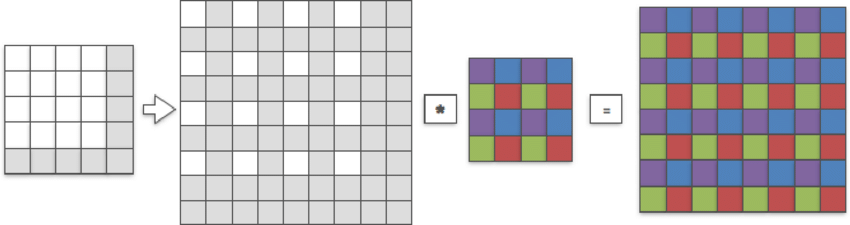
\includegraphics[width=\textwidth]{figures/neural_networks/subpixelconv1.png}
        \caption{Sub-pixel convolution as dilation then filtering.}\label{subfig:subpixdilate}
    \end{subfigure}
    \vskip\baselineskip
    \begin{subfigure}[b]{\subfigwidth}
        \centering
        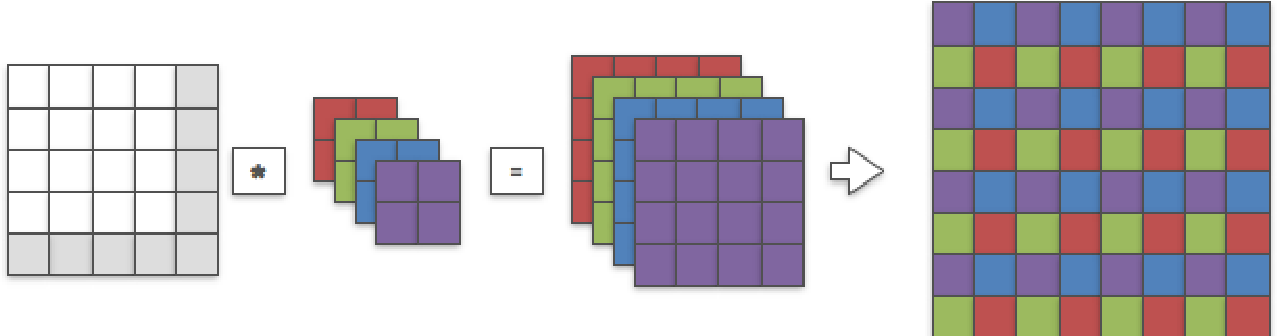
\includegraphics[width=\textwidth]{figures/neural_networks/subpixelconv2.png}
        \caption{Sub-pixel convolution as filtering then pixel-shuffling.}\label{subfig:pixelshuffle}
    \end{subfigure}
    \caption{Sub-pixel convolution.}\label{fig:subpixelconv}
\end{figure}